\documentclass{ximera}

\typeout{Start loading xmPreamble.tex}%

% Add here extra macro's that are loaded automatically by all documents of claas 'ximera' or 'xourse' in this repo

%%
%%  Example:
%%
% \newcommand{\R}{\mathbb{R}

\title{Lesson 1: Making Calculations (And Getting to Know the Layout)}
\begin{document}

\begin{abstract}
In this lesson, we will explore basic calculations and how to work with variables in MATLAB.
\end{abstract}
\maketitle

\section*{Activity 1: Getting to Know MATLAB}

In this activity, we'll cover basic calculations and how to work with variables in MATLAB. 
First, let's take a look at the setup of MATLAB. Feel free to reference these images as needed.

\subsection*{MATLAB Online Setup}

If you're using MATLAB Online, after opening up a live script your setup should look something like this:

\begin{center}
    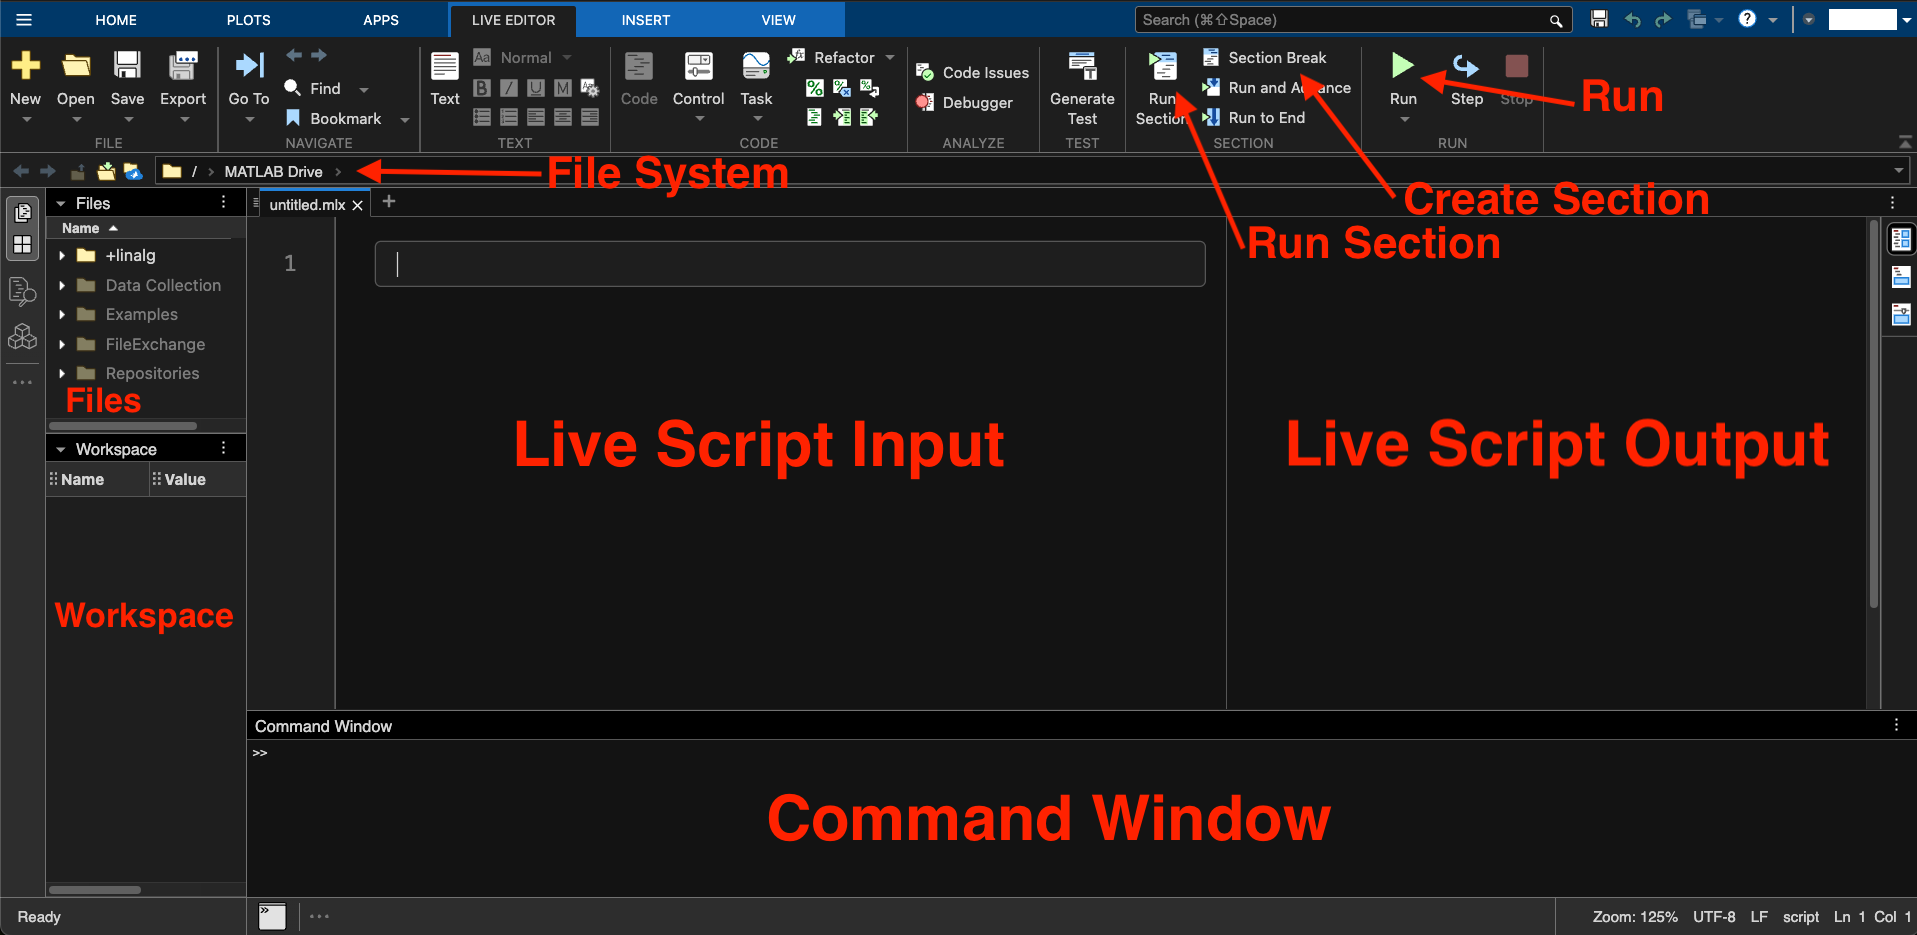
\includegraphics[width=0.8\textwidth]{MATLAB_Online.png}
\end{center}

\subsection*{MATLAB Downloaded Setup}

Within a live script, the interface will appear as follows. This window is separate from the command window and workspace.

% \begin{center}
% \includegraphics[width=0.8\textwidth]{matlab_downloaded_setup.png}
% \end{center}

The workspace and command window appear as follows:

% \begin{center}
% \includegraphics[width=0.8\textwidth]{matlab_workspace.png}
% \end{center}

\section*{Activity 2: Basic Calculations and Variables}

Let's start by performing some basic math operations. 

\begin{example}
Suppose you're driving a car and travel 100 meters in 20 seconds.
In the code below, type out the calculation that determines the speed of the car in meters per second.

\begin{remark}
\textbf{Note:} MATLAB ignores anything after a \texttt{\%} sign. This is called a \textbf{comment}, and you can use it to add notes. 
Comments can be placed on the same line as the code, and anything before \texttt{\%} is executed while anything after is ignored.
\end{remark}

\begin{verbatim}
% Use the "/" sign to divide 100 meters by 20 seconds
100 / 20
\end{verbatim}

This operation is similar to what you might enter in a graphing calculator.

To execute this command, select the \textbf{"Run Section"} button in the live script. MATLAB will run this computation, 
and the answer will appear on the right side of the screen labeled as \texttt{ans}.

\begin{remark}
\textbf{Note:} The large green \textbf{"Run"} button executes the entire live script from top to bottom, rather than just the selected section.
\end{remark}

You should see the following output \texttt{ans = 5}

(5 meters per second is approximately 11 miles per hour).
\end{example}

\section*{Workspace}
Now, check your \texttt{workspace}, it should contain \texttt{ans}. Note that the \texttt{Name} is \texttt{ans}, the \texttt{Value} is 5. If you hover over \texttt{ans} it will say \texttt{1x1 double}, and if you click on it a spreadsheet will appear called \texttt{ans} that has 5 in the first entry of the spreadsheet.

Calling 5 a \texttt{1x1 double} means that it is a single number (we'll have larger data entries later, like arrays and matrices), and the \texttt{double} means that it is stored as a decimal with \texttt{double} precision. We'll have some control over what kind of number or object is stored in the workspace.

\begin{example}
Now do the calculation to get the average speed of a car that's traveled 250 meters in 30 seconds.

\begin{verbatim}
%use the "/" sign to divide 250 by 30
\end{verbatim}

\begin{remark}
Note that again in the workspace there is still \texttt{ans}, but it has a value of 8.333.
\end{remark}

This replaced the previous \texttt{ans} with the new value.
\end{example}

If we name a value, it will create a new stored number in the workspace under that same name. We create named values by the syntax \texttt{name = value}

\begin{remark}
Note that we use a single equals sign when naming the variable. The equal sign acts as an indicator to MATLAB that you want to store the value as something different from \texttt{ans}, and then it reads the value and stores the named data point in the workspace.
\end{remark}

Notice in the code below, the quantity \texttt{distance\_1} is given a value of 100, using the syntax

\begin{verbatim}
distance_1=100
distance_1 = 100; % distance in meters
\end{verbatim}

\begin{remark}
Note: The semicolon \texttt{ ; } means that the data will be stored in the workspace, but it hides the output in the live script so that you don't see it. This will be more useful later.
\end{remark}

\begin{example}
Now, again calculate the speed of the car traveling 100 meters in 20 seconds, but call it \texttt{speed\_1} (Underscores help the names be readable by humans. Computers don't like spaces between words.)

First, name the time quantity \texttt{time\_1} and give it a value of 20. (We know the unit is seconds, but computers don't typically store units via code)

\begin{verbatim}
%name the quantity time_1 and give it a value of 20, using the syntax time_1=20
%name the quantity "speed_1" and calculate it based on the values distance_1 and time_1
\end{verbatim}

You should now see \texttt{distance\_1}, \texttt{time\_1}, and \texttt{speed\_1} in your workspace (and likely \texttt{time\_1} and \texttt{speed\_1} show up in your live script as outputs. It's nice to be able to reference values from the livescript as you progress).
\end{example}

\begin{example}
Now, make a \texttt{speed\_2} calculation for the car traveling 250 meters in 30 seconds. 

\begin{remark}
Note that MATLAB can only reference data that is in the workspace, so you usually want to first define your sections to be read from top to bottom. That is, first define distance and time, then define speed as relying on distance and time at the bottom of the section.
\end{remark}

\begin{verbatim}
%define distance_2 to have a value of 250
%define time_2 to have a value of 30
%define speed_2 as the ratio of distance and time
\end{verbatim}
\end{example}

\section*{Activity 3: Data as ``Variables''}

Each named quantity so far is called a \textbf{variable}. Variables can be all sorts of things (functions, matrices, vectors, symbols, text), as we'll see.

Some numbers and functions are automatically stored in MATLAB, like \texttt{pi} is an approximation of \(\pi\). The default stores \texttt{pi} as a double precision approximation of \(\pi\), so 3.1416. We'll learn later how to change the precision as desired. In general, the default precision is double.

\begin{example}
Approximate the area of a circle with radius 5 cm. 

Just like in calculators, \texttt{\^} is used for exponentiation (e.g. squaring, cubing, etc.), and \texttt{*} is multiplication.

The radius is given to be 5cm. Notice that the contextual comments are given after the variable definition. It's generally a good idea to comment often so that when you return to the code you have to spend less energy interpreting the code. For this same reason, it's a good idea to also use meaningful names for the variables (like \texttt{radius} and \texttt{area} instead of \texttt{a} and \texttt{b}).

\begin{remark}
Note: BEFORE RUNNING THE CODE: Pause and think about what you expect the output to be.
\end{remark}

\begin{verbatim}
radius = 5; % radius in cm
%define the variable "area" using ^ and *, 
%just as you would in a calculator. The area of a circle is pi times
%the radius squared.
\end{verbatim}
\end{example}

One major benefit of working with computational software, like MATLAB or Python, is that instead of storing and working with just one answer at a time, very very complex calculations can be performed in human-readable ways. We won't really see this benefit in this lesson, since we're just warming up and learning ways to make calculations, but we will see this benefit later on.

In the above code, even the fact that you can call the calculation \texttt{area} helps you think about what the number means for you in your work and in your analyses.

\begin{example} Calculate the exact area of the circle.

In MATLAB, you can take this one step further, by storing certain numbers or variables \textbf{symbolically}. This helps us as humans keep in mind the exact values that are being represented by our calculations. 

In this case, since \texttt{pi} is by default 3.1416, we can't actually calculate the exact value of the area using decimals.

If we again calculate the area, but want \(\pi\) to represent the irrational number, not an approximation, we can use \texttt{sym()} to have MATLAB represent \(\pi\) symbolically. We can then later make an approximation from this, but the new output will represent the exact area of the circle, not just a decimal approximation.

First, you'll see a symbolic output of \(\pi\), then you can use it to calculate \texttt{area\_sym}, the exact area of the circle.

\begin{remark}
Note: BEFORE RUNNING THE CODE: Pause and think about what you expect the output to be.
\end{remark}

\begin{verbatim}
sym(pi)
%Define a new variable called area_sym to be the area of the circle, but
%instead of pi, use sym(pi), as above.
\end{verbatim}

\begin{remark}
Note: The live script displays 25$\pi$, using the standard symbols, to represent the exact area rather than an approximation. This will be useful when we want MATLAB to expedite algebraic or other notational computations for us very quickly while maintaining the exact values of the quantities involved.
\end{remark}

\begin{remark}
Note: You can get back to the decimal using " double() "
\end{remark}

\begin{remark}
Note: BEFORE RUNNING THE CODE: Pause and think about what you expect the output to be.
\end{remark}

\begin{verbatim}
%type double(area) to get the same decimal approximation from earlier.
% "double()" will take an input and convert it to a decimal (if possible).
\end{verbatim}
\end{example}

Here are some other common symbols you might come across. 
\begin{remark}
Note: As they build in complexity, it is important to use sym() on the most basic building block of the quantity.
\end{remark}

First, \(e\) is stored as \texttt{exp(1)}, so \(e^x\) is \texttt{exp(x)}.

\begin{verbatim}
exp(1)
%use sym(1) to define "e" symbolically. 
%Now, instead write exp(sym(1))
\end{verbatim}

\begin{remark}
Note: exp(sym(1)) gave the desired symbolic number \(e\), whereas sym(exp(1)) gave a long fraction. This is because exp(1) is a decimal, which sym() converts to a fraction. Alternatively, sym(1) turns 1 into a symbolic number, and then exp(sym(1)) tells the system to do symbolic algebra.
\end{remark}

\section*{Activity 4: Making Symbolic Variables Nice}

\begin{remark}
Note: The same phenomenon appears below. Write sym() around the appropriate number to make the output a nice symbolic expression rather than a complicated fraction.
\end{remark}

\begin{remark}
Note: Here we are using "cos()" to take the cosine of a number, and "sqrt()" to take the square root of a number.
\end{remark}

\begin{verbatim}
sym(pi^2)
sym(cos(1))
sym(sqrt(pi))
\end{verbatim}

You should see the symbolic outputs \(\pi^2\), \(\cos(1)\), and \(\sqrt{\pi}\).

\section*{Activity 5: Stringing Multiple Calculations Together}

Now, let's take this one step further. You can think of simple volumes as extending a fixed area across a height. So, for a cylinder, its volume is computed by projecting a circular area across its height, as displayed below.

\begin{center}
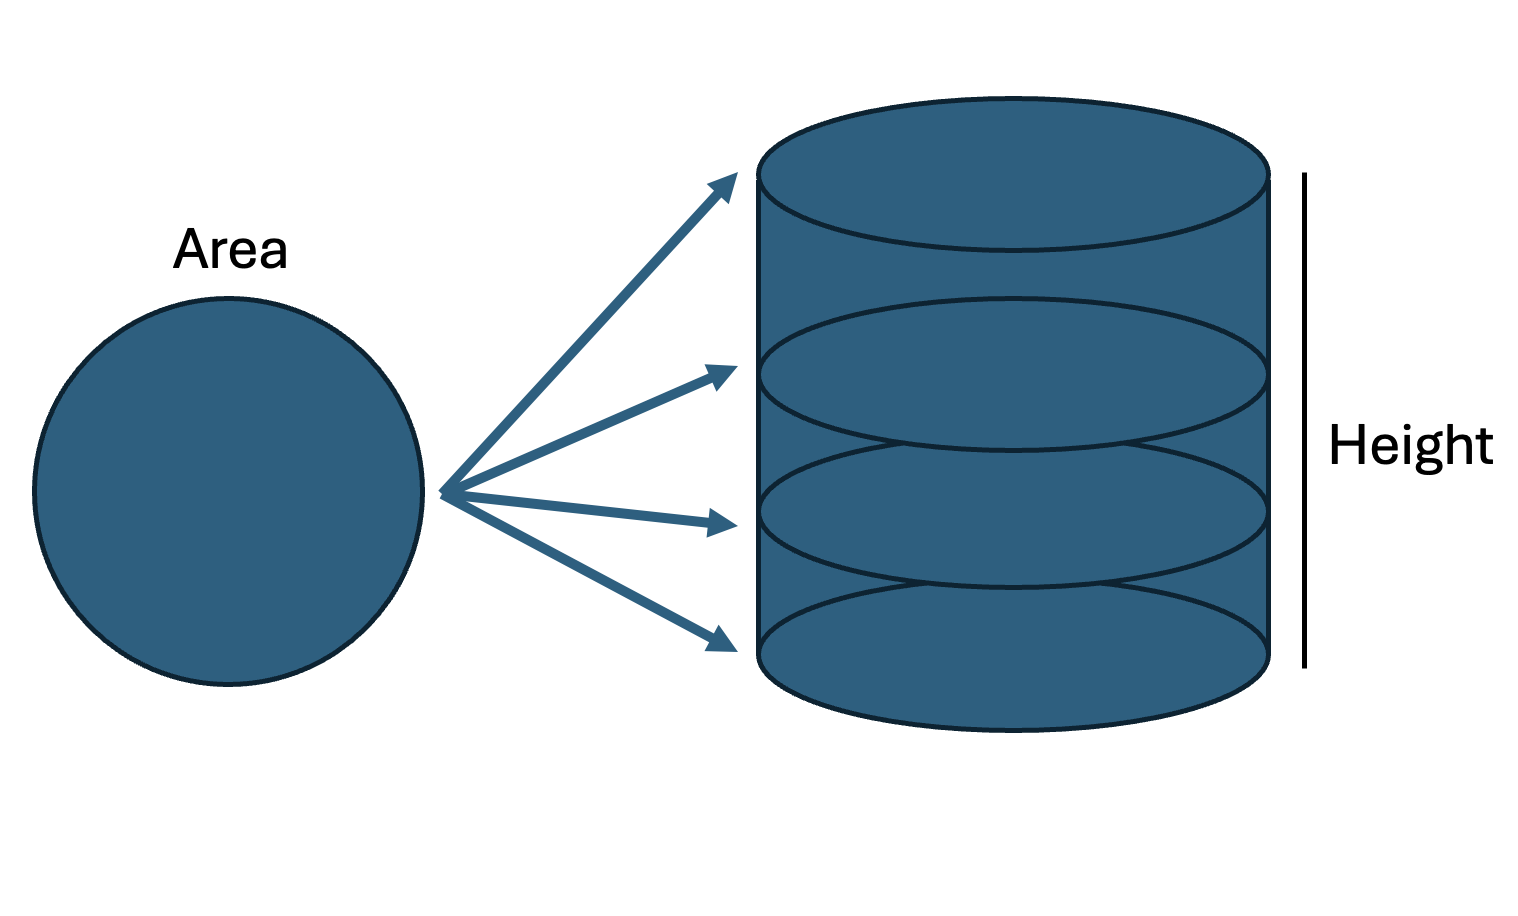
\includegraphics[width=0.4\textwidth]{Cylinder_Image.png}
\end{center}

\begin{example}
Now, using two lines of code and only words (i.e. named variables) in the final line of code, calculate the volume of a cylinder with circular cross-sectional area (radius 5) and a height of 10.

\begin{verbatim}
height=10; %defining the height, notice the semicolon hides the output.
%name a variable called "volume" that gives the volume of the cylinder,
%using only words and operations (+, -, *, ^,/)
%NOTE: area is already defined in the sections above, and is already in
%your workspace so you don't need to define it again.
\end{verbatim}

You should see either \texttt{volume = 785.39...} or \texttt{volume = 250} depending on your setup.
\end{example}

\section*{Activity 5: Computing Measures of Quantities}

\textbf{Some Helpful Definitions, Formulas, and Descriptions}

For the remainder of the course, we will be making calculations using MATLAB to compute the values of various quantities. Usually the quantities are physical. You'll be solving problems and making interpretations as you go, so it is important to ground your understanding of the ideas in some basic definitions, and to use some basic formulas.

The following are descriptions of the fundamental ways we think about and quantify various important quantities. For now, assume that all of these quantities have constant measures (meaning they don't change). This is why the "approximation" symbol is used; many of the following quantities are not necessarily constant, but for now we will roughly treat them as such.

\begin{enumerate}
    \item \textbf{Mass}, loosely conceived, is a measure of "how much matter" is within an object. We will use the "gram" unit, denoted by \texttt{g}. More specifically, the "kilogram" \texttt{kg} is 1000 grams.
    
    \item An object's \textbf{volume} is a measure of how much space an object occupies in our 3D world. If we break up our world into three dimensions (say, "length", "width", "depth"), then the volume of an object can be loosely thought of as the product of its three dimensions (so $\text{volume} \approx \text{length} \times \text{width} \times \text{depth}$), even though only blocks' (rectangular prisms) volumes can be directly measured through this product. Because of this three-part product (called "cubing"), the unit of volume is $m^3$ (cubic meters).

    Common volume measures:
    \begin{itemize}
        \item Sphere with radius $r$: $V = \frac{4}{3} \pi r^3$
        \item Cone with base radius $r$ and height $h$: $V = \frac{1}{3} \pi r^2 h$
        \item Pyramid with a base of area $A$ and height $h$: $V = \frac{1}{3} A h$
    \end{itemize}

    Note that each of these measures are cubic in nature, even though they are not explicitly $l \cdot w \cdot h$.

    \item An object's \textbf{density} is the comparative measure of mass and volume. That is, "how much matter" is in the object relative to "how much space it takes up". For this relative, comparative measure, we use division: $\text{density} = \frac{\text{mass}}{\text{volume}}$, and it has units $g/cm^3$ or $kg/m^3$.

    \item \textbf{Distance} between two objects is an intuitive quantity. It measures "how far apart" two objects are in space. Here, the "far apart" is measured by the length of a straight line drawn between the objects. Because length is one-dimensional, it has the unit $m$ (meters).

    \item An object in motion is traveling some distance over a period of time. That object's \textbf{velocity} is the relative comparison of its distance traveled and the time of travel. Velocity is measured by the ratio $\frac{\text{distance}}{\text{time}}$, in units $m/s$ (meters per second).
\end{enumerate}

\begin{remark}
Note: The units can change scales pretty fluidly, as long as you are consistent. Sometimes it makes the numbers easier to just work in grams, or in meters per minute, or in deca-meters per second (1 deca-meter is 10 meters).
\end{remark}

\section*{Task: Computing Measures of Quantities in MATLAB}

With the above definitions in mind, compute the following measures of quantities using MATLAB to make the calculations. Try to calculate each quantity using multiple lines, where the first few lines name relevant values necessary for the quantity calculation (e.g. \texttt{distance}, \texttt{time}, \texttt{height}, \texttt{width}) and then the final quantity is defined only through computations (+, -, /, *, \^{}) and words (e.g. \texttt{density}, \texttt{volume}, etc.)

\subsection*{Problems:}

\begin{enumerate}
    \item Rank masses of the objects from largest to smallest. All objects will have a radius of the same length, 5.
    \begin{enumerate}
        \item A cone with height 5, density $2.5\ g/cm^3$
        \item A sphere with a density of $1.9\ g/cm^3$
        \item A cylinder with a height of 8 and a density of $3.1\ g/cm^3$
    \end{enumerate}

    \textbf{BEFORE RUNNING THE CODE:} Pause and think about what you expect the output to be.

    \begin{verbatim}
% First, define a "radius" variable with a value of 5. Each of the shapes
% share the same radius, so you should only need one radius defined for all
% of the shapes.
% Then, construct each mass so that you can compare their outputs.
    \end{verbatim}

    Your calculations should reveal that \texttt{mass\_cylinder > mass\_cone > mass\_sphere}.
    
    \item It takes Jenny 30 seconds to reach point A at a speed of $3\ m/s$, 19 seconds to reach point B at a speed of $5\ m/s$, and 50 seconds to reach point C at a speed of $2\ m/s$. Which object is farthest from Jenny?

    \textbf{BEFORE RUNNING THE CODE:} Pause and think about what you expect the output to be.

    \begin{verbatim}
% Use the speeds and times to calculate the distances for comparison.
    \end{verbatim}

    Your calculations should reveal that \texttt{point C is farthest}, even though \texttt{its speed is lowest}.
\end{enumerate}

\section*{Activity 6: Comparing Written Code}

The following are different lines of code produced to answer the following question:

\textbf{Question:} Calculate the sum of the masses of a sphere with radius 7 m and density $10\ kg/m^3$ and a cone of radius 8 m, height 2 m, and density $25\ kg/m^3$.

\subsection*{Code 1}

\begin{verbatim}
3.14*(10*1.333*343+64*50/3)
\end{verbatim}

\subsection*{Code 2}

\begin{verbatim}
r_sphere=7;
density_sphere=10;
volume_sphere=4/3*pi*r_sphere^3
mass_sphere=density_sphere*volume_sphere

r_cone=8;
h_cone=2;
density_cone=25;
volume_cone=1/3*pi*r_cone^2*h_cone
mass_cone=volume_cone*density_cone

total_mass=mass_sphere+mass_cone
\end{verbatim}

\subsection*{Reflect:}
Keeping in mind that these are extreme examples, reflect and comment on:

\begin{enumerate}
    \item The similarities and differences between the codes.
    \item The benefits and drawbacks of each code.
    \item What it would take for a person to revisit the code after its writing and understand what the code does and if it accomplishes the goal.
    \item How do you explain differences in output of the code?
\end{enumerate}


\end{document}